\chapter{Studies of environmental noise during O3}\label{ch:noise-studies}

{\color{red}
Introduce how observing/engineering runs work, O3 schedule, etc.}

\ac{O3} was preceded by an engineering run, a month-long period during with the interferometer is operational at low-noise levels but not observing \ac{GW} events, to provide time for detector commissioning and noise studies.

\section{Evaluation of coupling functions}\label{sec:evaluation-of-cf}

{\color{red}
Pretty much just copied from PEM paper.
Goal is to include most or all of the referenced calculations and figures here.}

Before discussing results of injection studies and coupling function measurements in \ac{O3}, it is necessary that we take a moment to assess how well they estimate excess noise in the interferometer when the noise source is known to be the result of environmental coupling.
Of course, one could do this by applying coupling functions to a set of ``test'' injections, but this would require performing more injections, which as mentioned before is typically not feasible.
Furthermore, since the intention of the coupling functions is to estimate the impact of noise signals originating from a broad variety of sources, it make sense to use non-laboratory signals when evaluating coupling estimates.
Therefore, we use noise events not produced by injection equipment to evaluate how accurately the coupling functions recover the actual excess noise observed in the \ac{GW} strain data.

Thunderstorms are known to produce short-duration transients in the strain data at tens of Hz.
At \ac{LLO}, coupling functions for several accelerometers at the Y end station, where vibrational coupling was the highest, are capable of estimating the amplitude of multiple noise transients to within a factor two during a particularly loud thunderstorm~\citep{alog_thunder}.

Helicopter flyovers can produce narrow-band features up to tens of seconds long.
Coupling functions of various sensors at both observatories can predict the amplitudes of lines produced by multiple helicopter flyovers during O3 to within a factor of two in most cases~\citep{alog_helicopter}.

Long-duration noise due to vibrations from rain and the building \ac{HVAC} is also well characterized by coupling functions at \ac{LHO}~\citep{alog_rain, alog_hvac_coupling}.

\section{Vibrational noise studies during O3}\label{sec:vib}

\begin{figure}[h!]
	\centering
	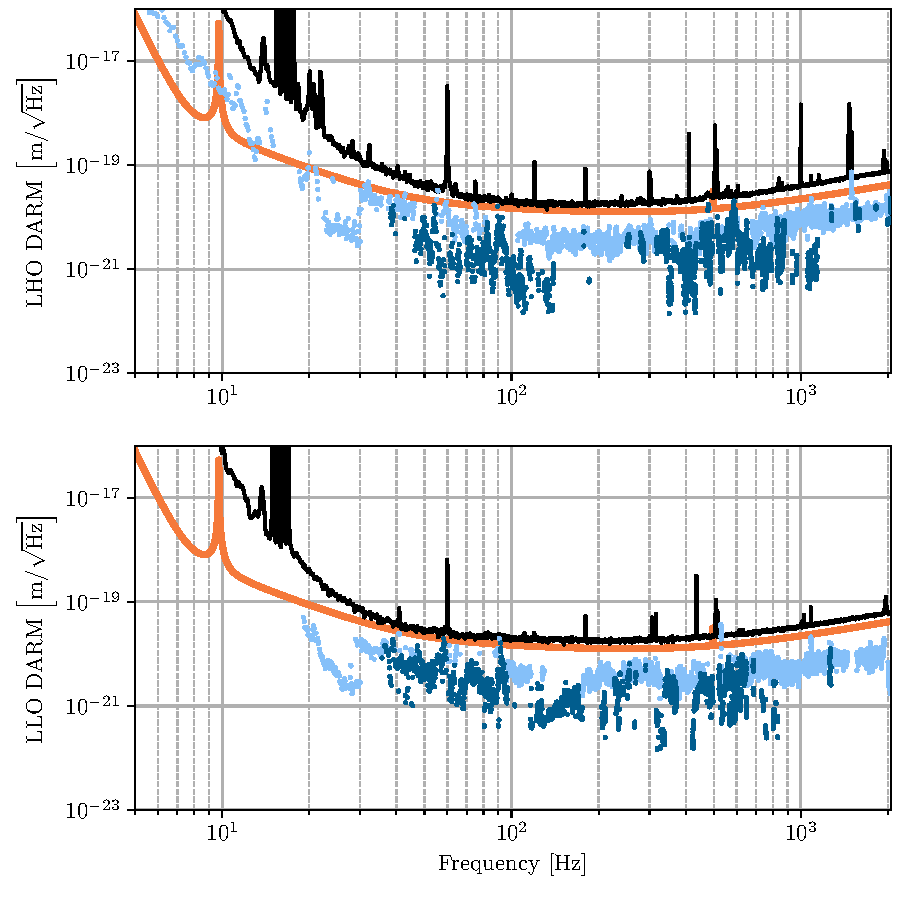
\includegraphics{figures/noise-studies/vib-ambient.pdf}
	\caption{
		Ambient estimate of vibrational noise levels at LHO (top) and LLO (bottom).}
	\label{fig:vib-ambient}
\end{figure}

Figure~\ref{fig:vib-ambient} shows the ambient contribution of vibrational noise during \ac{O3}, produced by combining the highest coupling factors among accelerometers and microphones measured from an injection campaign at the beginning of \ac{O3}.
At the end of \ac{O3}, the vibration noise background at both observatories was dominated by input beam jitter above 100\,Hz (discussed in Section~\ref{sec:vib-septum}).
At \ac{LHO},  the dominant coupling region below 100\,Hz was the output arm.
At \ac{LLO}, the dominant coupling regions were the Y-end in the 40-60\,Hz band and the output arm in the 60-100\,Hz band.

\subsection{Scattered light at the HAM5/6 septum}\label{sec:vib-septum}

At \ac{LHO}, investigations throughout \ac{O3} showed that scattering noise produces noise near the detector noise background in the frequency range of 38--100\,Hz.
The sensors with the highest ambient projections in this band were accelerometers located on the HAM 5 and HAM 6 vacuum chambers, which contain the \ac{GW} channel readout, as well as the optics of the output mode cleaner, squeezed light system, and signal recycling cavity.
The coupling was excited most strongly by injections around the output arm, but acoustic noise produced as far as the Y-arm manifold $\approx 50$\,m away produced excess noise in \ac{DARM}.
Spectra from the nearest injections also show non-linear coupling behavior ({\color{red}Expand on this}).
Shaker injections were also performed throughout the corner station, confirming that the dominant coupling site was in the HAM 5 and 6 area.
This evidence suggested that the coupling was caused by scattered light within HAM 5 or HAM 6.
A more thorough investigation was required to localize the exact scattering surface.

Figure~\ref{fig:vib-impulse} shows time series and spectrograms of a single impulse injection performed in the \ac{HAM} 5/6 area.
The plots show a single impulse injection signal in the \ac{GW} channel and in various output optics accelerometers.
Multiple sensors observe an impulse time-of-arrival matching that of the \ac{GW} channel, but repeating the injection from various other locations rules out sensors that do not match it consistently across multiple injections.
In this case the septum (separating the HAM5 and HAM6 chambers) accelerometer signal matches the \ac{DARM} signal most consistently (other injections not shown for brevity).

Spectrograms of the same impulse injection for \ac{DARM} and the three sensors with the closest matching time-of-arrival to that of \ac{DARM} reveals similarities between the frequency structure of the septum accelerometer signal and that of \ac{DARM}.
This provides further support that the septum is the dominant coupling site in the output arm.

\begin{figure}[h!]
	\centering
	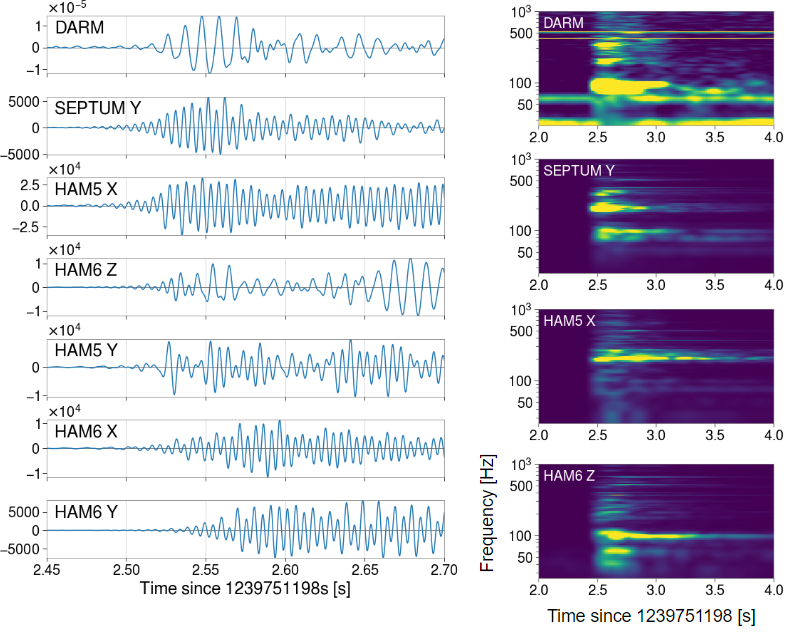
\includegraphics[width=\textwidth]{figures/noise-studies/vib-impulse.png}
	\caption{
		Time series (left) and spectrograms (right) of a vibrational impulse injection produced at the output arm of the LHO detector.}
	\label{fig:vib-impulse}
\end{figure}



\subsection{Search for the source of a 48-Hz peak}\label{sec:vib-48hz}

Figure~\ref{fig:vib-beat-spectrograms} shows spectrograms of a beating-shakers injection used to localize the coupling site responsible for a 48\hyp Hz noise peak in the \ac{DARM} spectrum.
The shakers were injecting at 48 and 48.01\,Hz. The Y-axes of the spectrograms are centered along at 48\,Hz and show the combined signal in each sensor modulating at the beat frequency (0.01\,Hz).
This set of spectrograms suggests that the accelerometers on the \ac{ITM} chambers and the Y-axis HAM2 accelerometer are likely not close to the true coupling location, since the beat envelopes are the furthest offset from the beat envelope in the \ac{DARM} response.

\begin{figure}[h!]
	\centering
	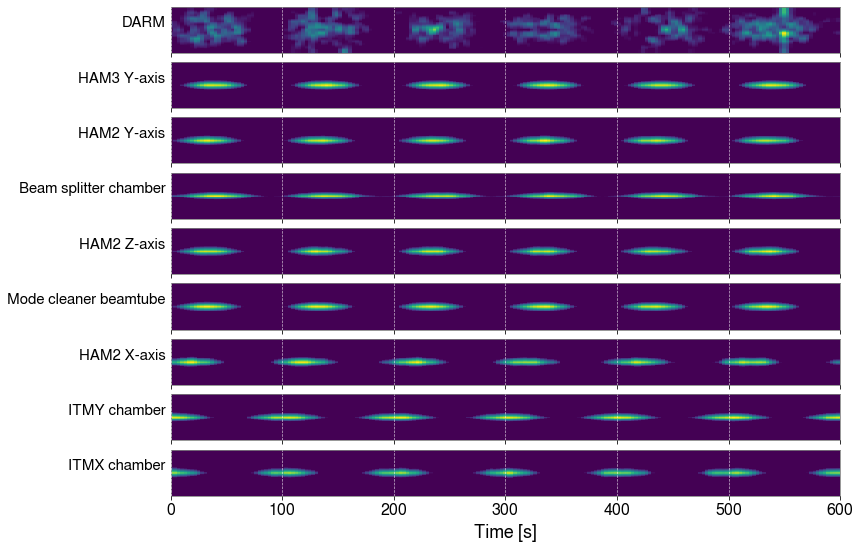
\includegraphics[width=\textwidth]{figures/noise-studies/vib-beat-spectrograms.png}
	\caption{
		Spectrograms of DARM and various accelerometers near the input arm and beam splitter showing a beating-shakers injection at 48\,Hz.}
	\label{fig:vib-beat-spectrograms}
\end{figure}

Multiple other injections were made (not shown here) with varying shaker locations in order to rule out other sensors until the most likely candidate remaining was the HAM3 Y-axis accelerometer.
Black glass was used to block scattered light at this location and the peak was eliminated for the second half of the O3 observation run.
Figure~\ref{fig:vib-48hz} shows the noise reduction in the \ac{GW} channel after the light scattering was mitigated.

\begin{figure}
	\centering
	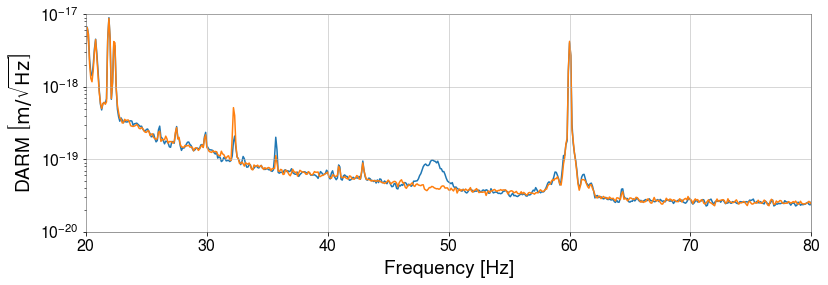
\includegraphics[width=\textwidth]{figures/noise-studies/vib-48Hz.png}
	\caption{LHO DARM spectrum before and after mitigation of the 48-Hz peak.}
	\label{fig:vib-48hz}
\end{figure}

\subsection{Input beam jitter}\label{sec:vib-jitter}

{\color{red}
Short discussion, summarize measurements and improvement.
Will make sure to discuss impact of test mass defect on jitter noise.}

\begin{figure}
	\centering
	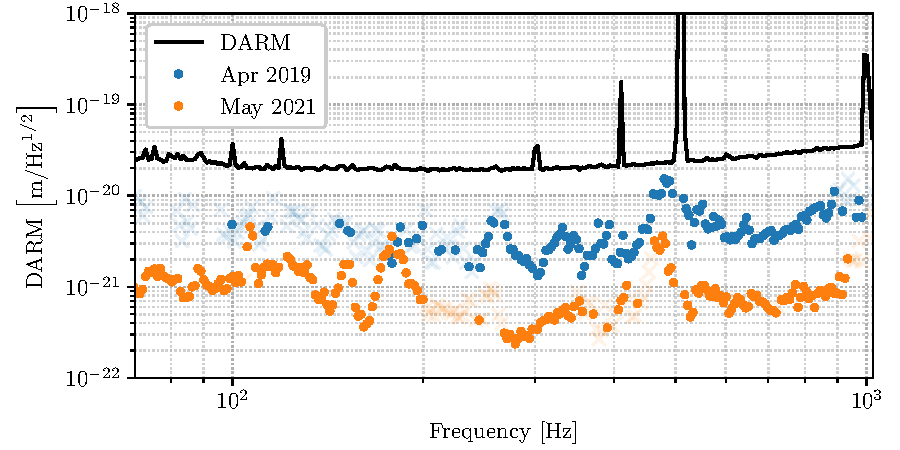
\includegraphics{figures/noise-studies/noise-jitter.pdf}
	\caption{Improvement in jitter coupling at LHO between the start and end of O3.}
	\label{fig:vib-jitter}
\end{figure}

\section{Magnetic noise studies during O3}\label{sec:mag}

\begin{figure}
	\centering
	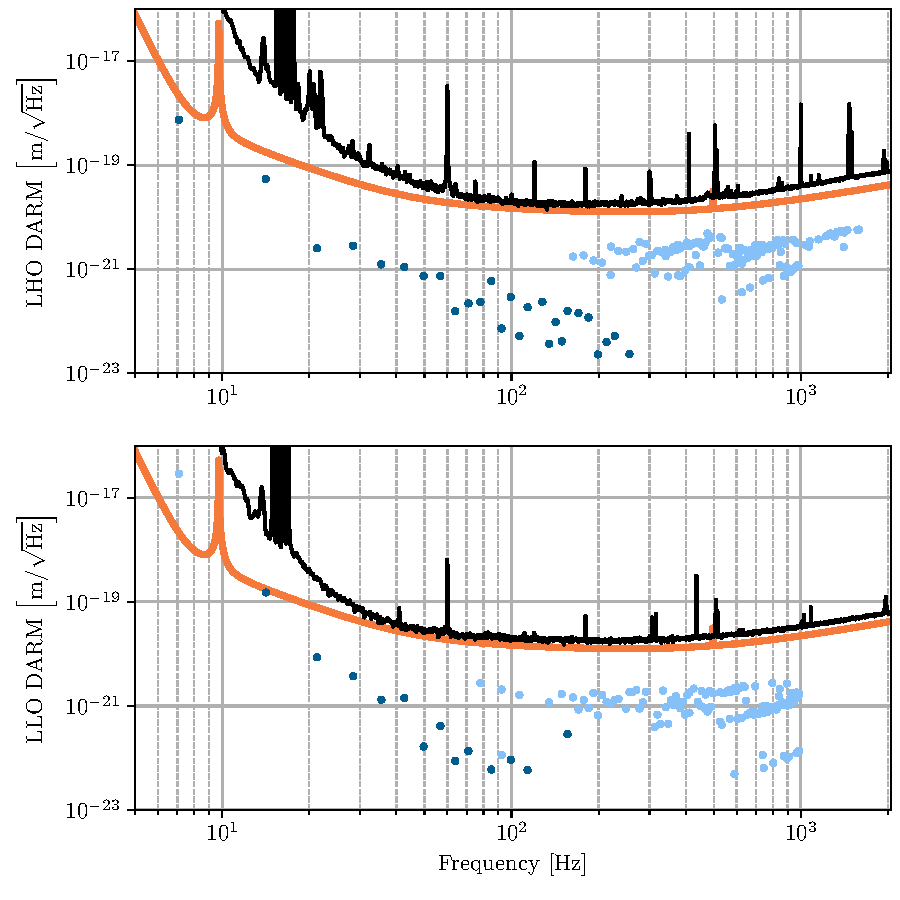
\includegraphics{figures/noise-studies/mag-ambient.pdf}
	\caption{
		Ambient estimate of magnetic noise levels at LHO (top) and LLO (bottom).}
	\label{fig:mag-ambient}
\end{figure}

Magnetic injections early in \ac{aLIGO} suggested that coupling to permanent magnets in the suspension system  could prevent \ac{LIGO} from reaching design sensitivity in the 10-20\,Hz regions~\citep{Schofield_2013}.
While the test mass actuator is electrostatic and not magnetic (as in \ac{iLIGO}), a number of permanent magnets were used in the suspensions, including for actuation in the first three of the four levels of the isolation chain and for eddy current damping.
The greatest number of permanent magnets were in the eddy current damping arrays and these were removed.
Nevertheless, ambient fields are still predicted to produce noise at greater than one-tenth of the design sensitivity in the 10-20\,Hz band (Figure~\ref{fig:mag-ambient}), and may need to be further addressed as we reach design sensitivity in the 10\,Hz region.

At higher frequencies, generally above about 30\,Hz, the dominant magnetic coupling appears to be through induction of currents in cables and at connectors, mainly to actuator cabling and other cabling in the control system.
Mitigation of coupling to cables and connectors has required a continuing program of monitoring coupling since cables are often disconnected and reconnected during runs as electronics are replaced for problems or upgrades.
This program consists of making weekly, broadband magnetic field injections using the large wall-mounted coils described in Section~\ref{sec:injections-magnetic}.
Since the injections are scheduled for every Tuesday morning before the routine detector maintenance period, the interferometer may or may not be in a locked state at the time, so an injections were not always performed.

\begin{figure}
	\centering
	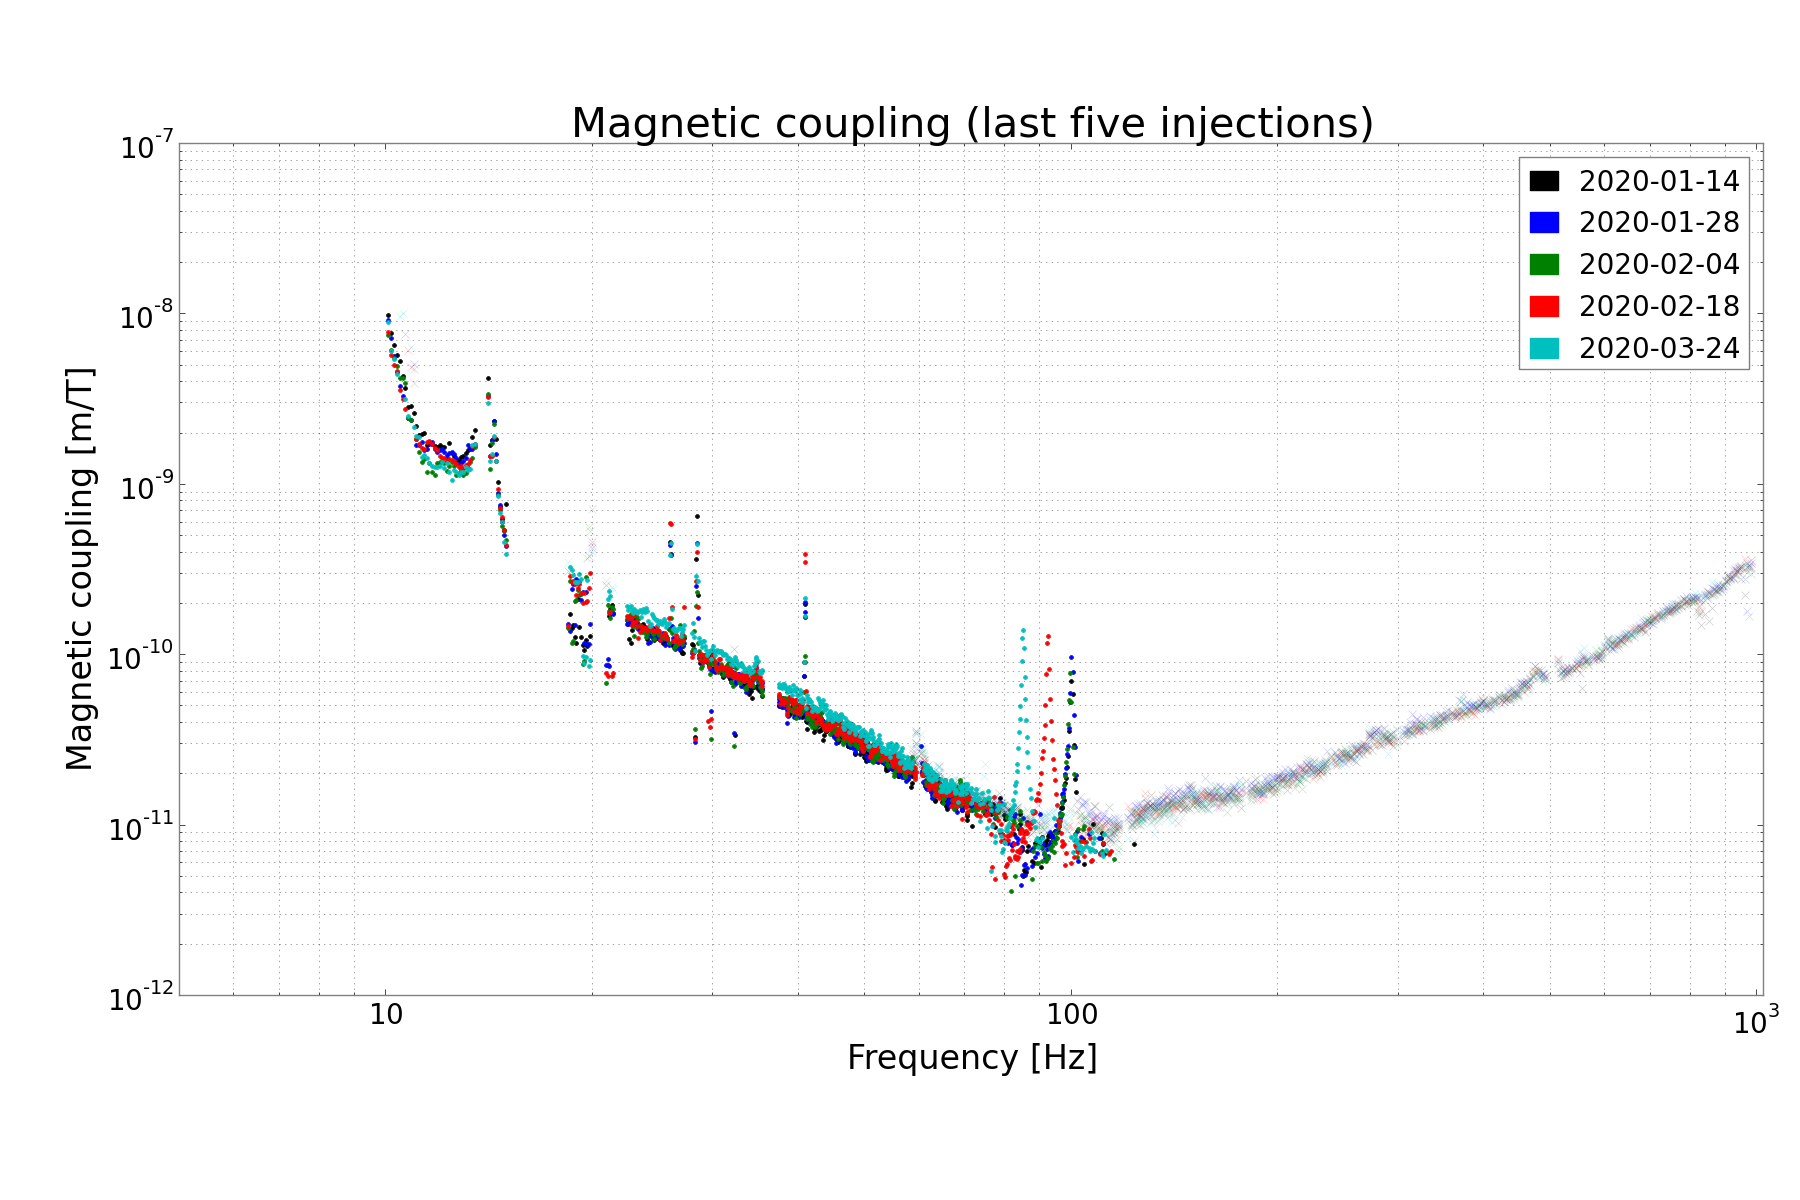
\includegraphics[width=0.9\textwidth]{figures/noise-studies/mag-weekly-cf.png}
	\caption{
		LHO magnetic coupling measured by the last five wall-mounted coil injections performed in O3.}
	\label{fig:mag-weekly-cf}
\end{figure}

Figures~\ref{fig:mag-weekly-cf}, \ref{fig:mag-weekly-bands}, and \ref{fig:mag-weekly-peaks} are automatically generated every week by the code that analyzes the injections.
The first of these shows magnetic coupling functions measured over the last five weeks for which a broadband injection was performed.
At this point a single injector was implemented at each of the three stations at LHO; the coupling functions show the highest coupling per frequency bin between the three stations.
Changes can be seen in both the broadband and narrowband structure of the coupling function.
Just within these five weeks, the level of broadband coupling varied by as much as a factor of about 1.5.
Since the injection is produced from a same location and at the same amplitude every time, uncertainties due to the injection source as discussed in Section~\ref{sec:uncertainties} do not account for these variations.
Broadband changes over specific frequency ranges tracked over the full course of \ac{O3} (Figure~\ref{fig:mag-weekly-bands}) show significant fluctuations throughout the run.

\begin{figure}
	\centering
	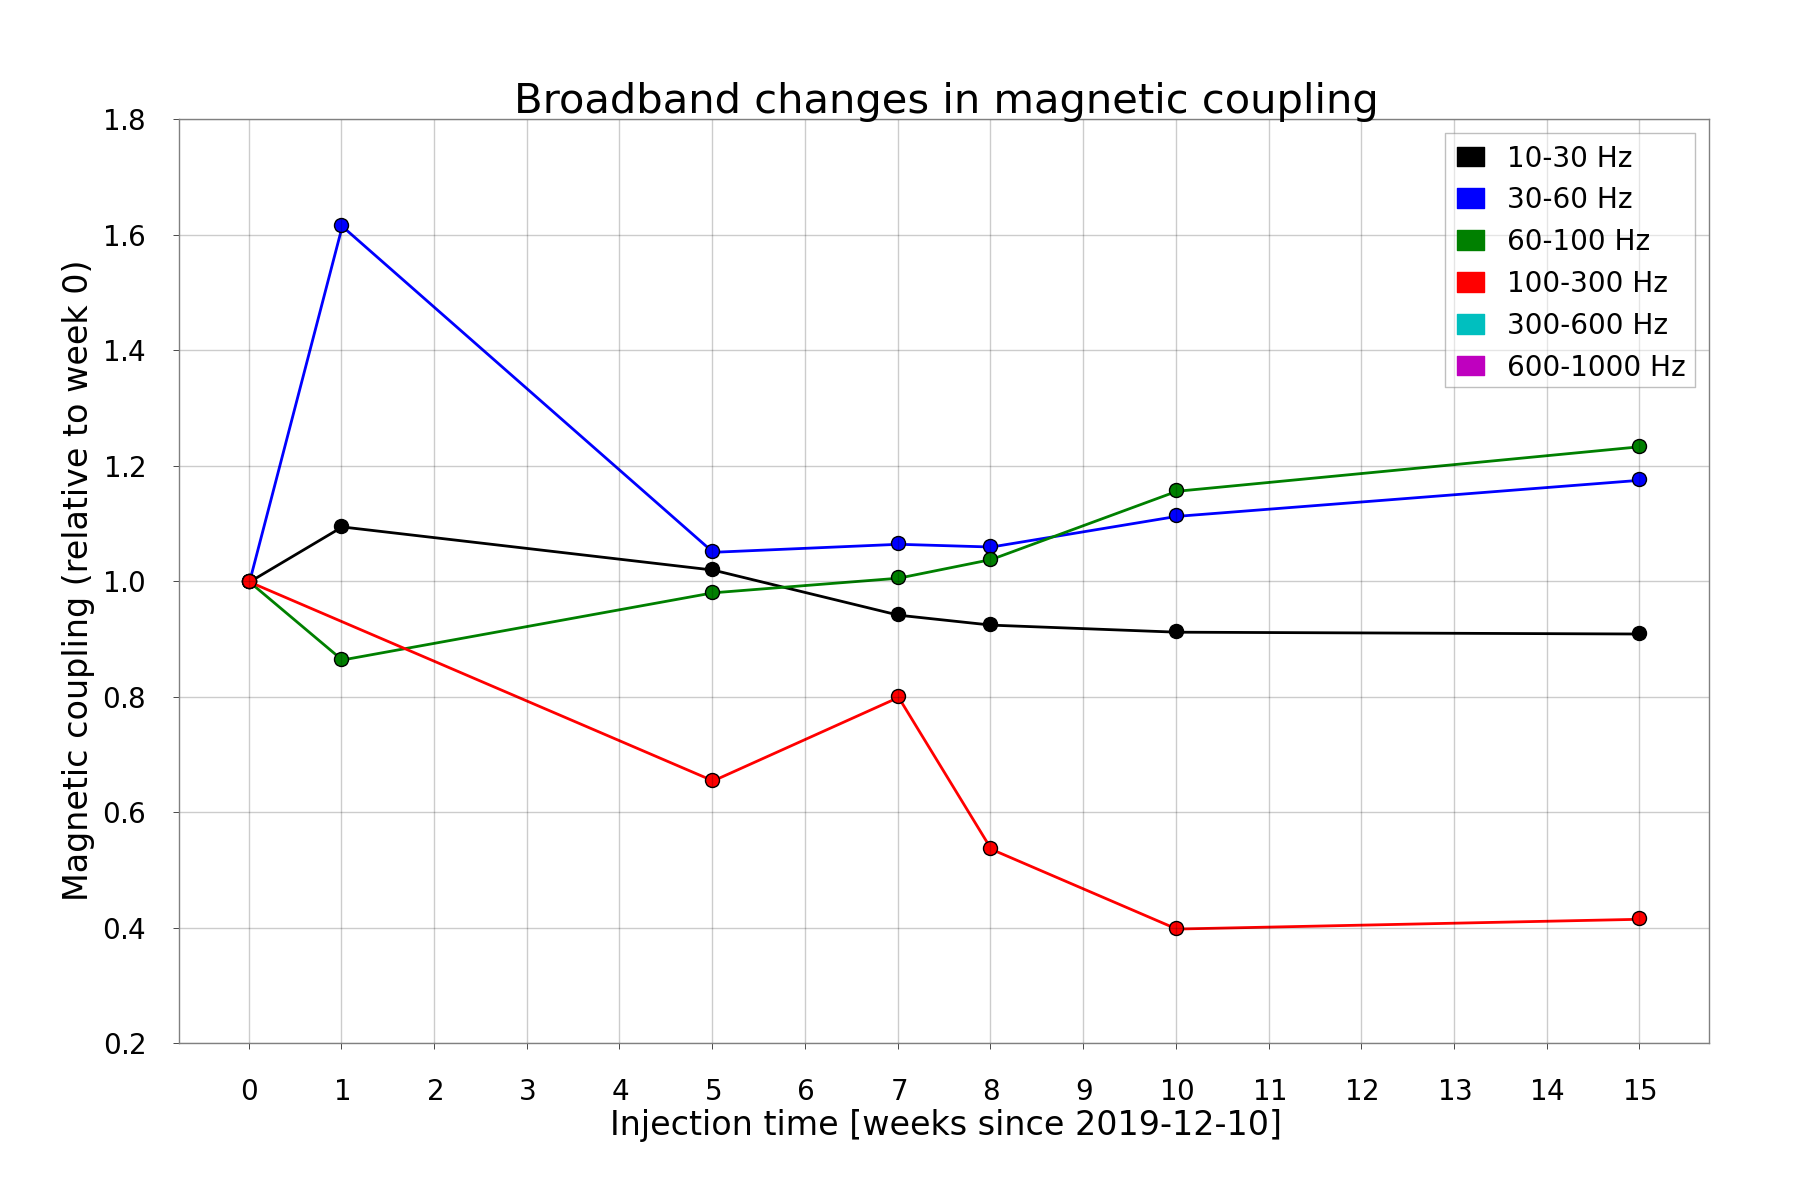
\includegraphics[width=0.9\textwidth]{figures/noise-studies/mag-weekly-bands.png}
	\caption{Time-lines of magnetic coupling changes relative to the start of the observing run.}
	\label{fig:mag-weekly-bands}
\end{figure}

Furthermore, a large peak in the coupling is seen migrating between 90 and 110 Hz.
This is precisely the type of feature often missed by comb injections but will be routinely discovered by broadband injections in future observing runs.
Figure~\ref{fig:mag-weekly-peaks} shows frequency and amplitude fluctuations in coupling peaks such as this.
Although the coupling of the $\sim100$\,Hz peak is still well below the level that would produce excess noise in the \ac{GW} channel, its presence gives reason to be concerned that similar peaks could arise in the future that do couple significantly.
These weekly injections would help in identifying when the coupling changed, so instrumentalists can deduce what changes to the electronics may have affected it.

\begin{figure}
	\centering
	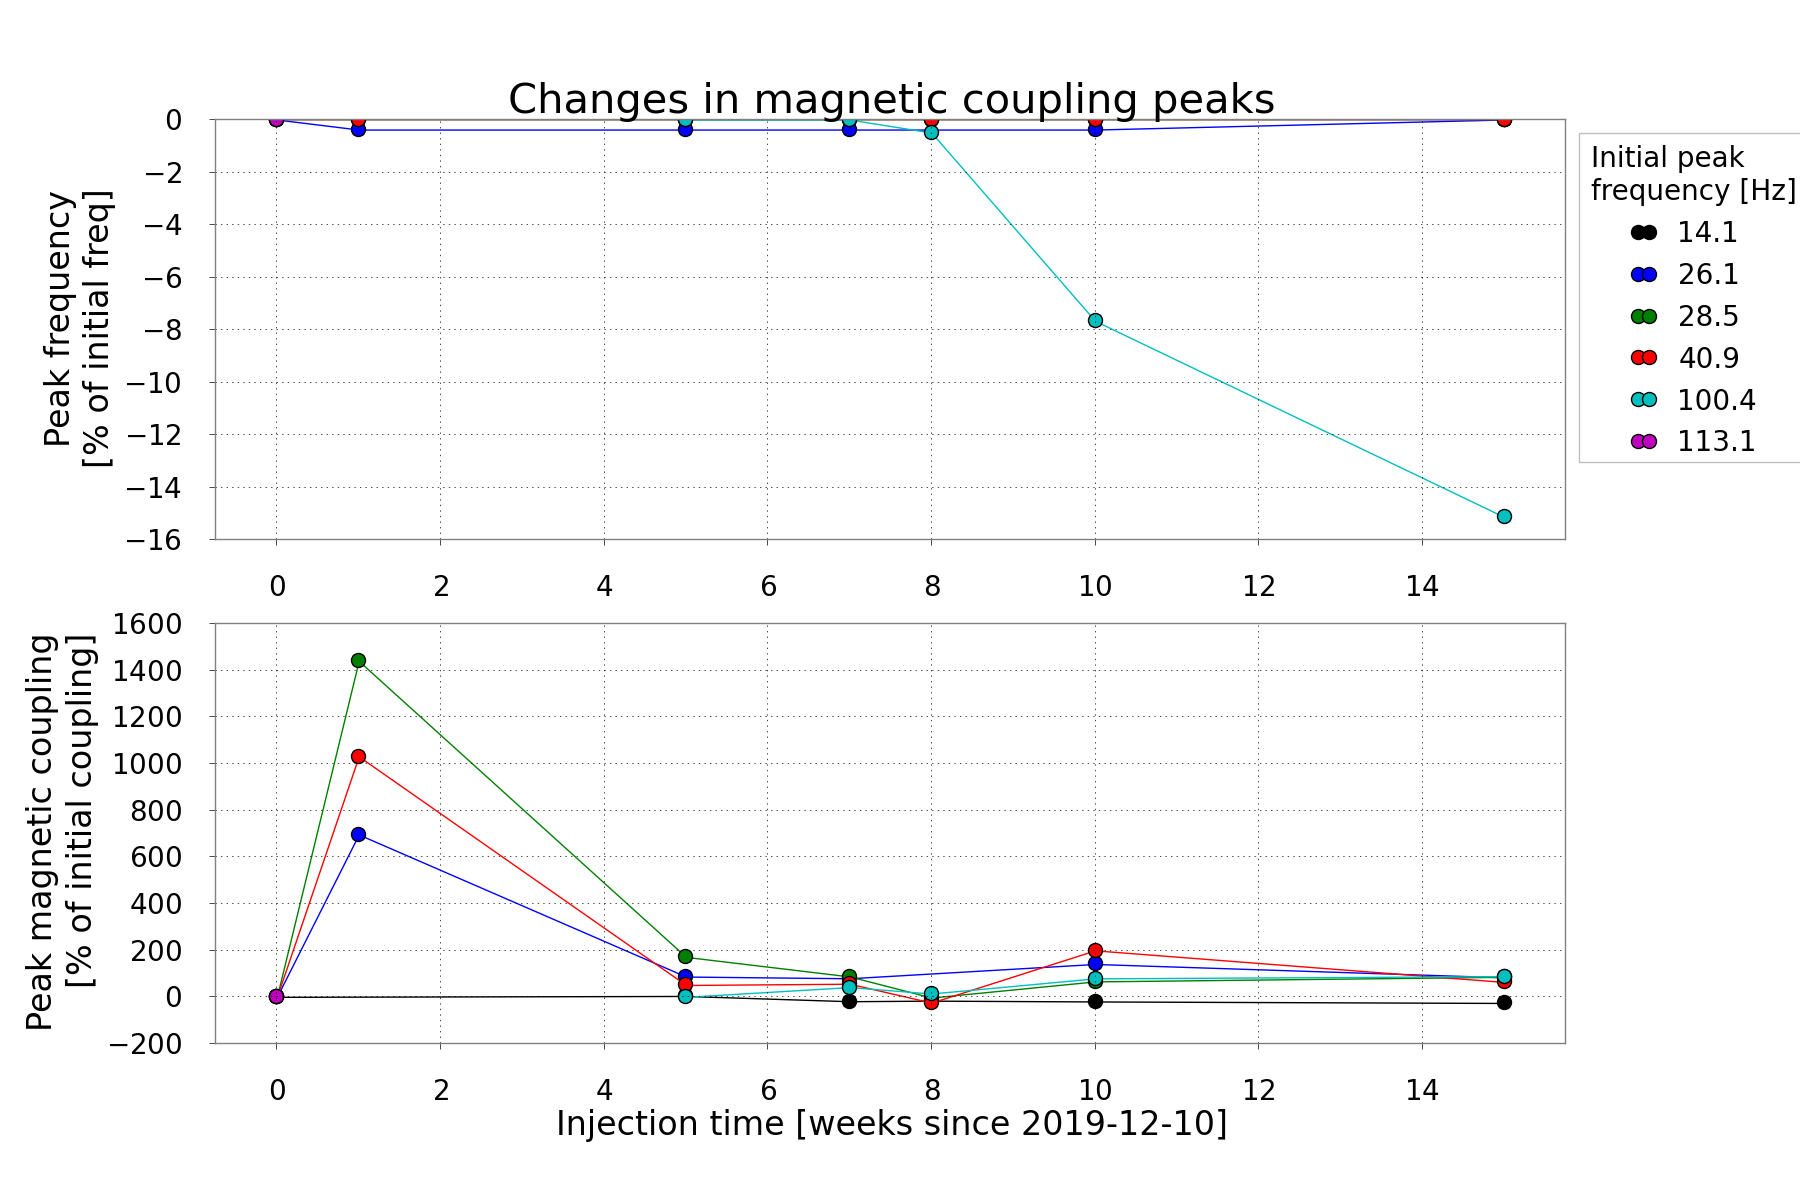
\includegraphics[width=0.9\textwidth]{figures/noise-studies/mag-weekly-peaks.png}
	\caption{Weekly trends in frequency (top) and amplitude (top) of peaks in the magnetic coupling functions.}
	\label{fig:mag-weekly-peaks}
\end{figure}

\section{Validation of gravitational wave event candidates}\label{sec:vetting}

In addition to investigating sources of environmental influences, knowledge acquired from environmental studies contributes to the vetting of \ac{GW} event candidates.
Analysis pipelines search the strain data for astrophysical signals.
They are categorized into modeled searches for binary mergers that match the data to template waveforms (e.g. GstLAL~\citep{Cannon_2012} and PyCBC~\citep{Usman_2016}) and unmodeled searches that identify excess energy coherent between multiple detectors (e.g. cWB~\citep{Klimenko_2008}, oLIB~\citep{Lynch_2017}, and BW~\citep{Cornish_2015}).

Contamination of the \ac{GW} data can occur through any of the means discussed in previous sections.
Environmental noise has the potential to be correlated between detectors by stemming from a common source, such as through electromagnetic signals from distant sources or glitches in GPS-correlated electronics.
The analysis pipelines estimate the false-alarm probabilities for \ac{GW} events based on the background rate of randomly coincident events in the detector network.
They generate background events by time-shifting the data stream of one detector relative to another by time steps much longer than the light travel time between detectors and longer than the duration of \ac{GW} signals.%~\citep{Was_2009}.
This method does not account for the possibility of transients being correlated between the detectors due to a common environmental source.

Environmental noise is also particularly relevant to unmodeled searches. Unlike template-based methods, these searches make minimal assumptions about the signal waveform and rely more heavily on signal correlation between sites.

The first observation of a \ac{GW} occurred on 14 Sept 2015~\citep{gw150914}.
The event, a short-duration binary black hole merger designated GW150914, required a number of follow-up investigations to find potential noise sources around the time of the event~\citep{Detchar_2016}.
This included an examination of the status of all \ac{PEM} sensors and any significant signals they observed for possible contamination of the GW signal~\citep{Schofield_150914}.
A few of the \ac{PEM} sensors were not working, but because of redundancy, coverage was sufficient.

Comparisons between Q-transform spectrograms~\citep{Chatterji_2004} of all coincident events in environmental sensors to the time-frequency path of the event revealed that no environmental signals had paths similar to the event candidate.
Q-transforms produce a quality-factor-optimized logarithmic tiling of the time-frequency space, making them useful for visualizing transients.
The \acp{SNR} of the matching signals were also compared to that of the event, showing that even if there were overlapping time-frequency paths, none of the environmental signals were large enough to influence the strain data at the \ac{SNR} level of the event, based on multiplying the environmental signals by their respective sensor coupling functions.

The validation process for novel events such as GW150914 also includes redundant checks for global sources of environmental noise.
We use a dedicated cosmic ray detector located below an input test mass at \ac{LHO} to examine any association of cosmic ray showers to excess noise in \ac{DARM}.
We also check external observatories for coronal mass ejections, solar radio signals, geomagnetic signals, and \ac{RF} signals in the detection band as well as higher frequencies.

There was specific concern over a co-incident extremely-high current (504\,kA) lightning strike over Burkina Faso, prompting additional studies of the effects of lightning on the interferometer~\citep{Schofield_lightning}.
Investigations of similar strikes found no effect on the strain data and investigations of closer strikes confirmed that the magnetometers were much more sensitive to lightning strikes than the interferometer was.
In conclusion there was no reason to veto the first detection based on environmental disturbances.

Subsequent detections throughout \ac{O1} and \ac{O2} employed a similar procedure; however the development of the method described in Section~\ref{sec:cf} for producing coupling functions for all sensors expedited the process.
This was especially important for examining environmental noise during GW170817, the first long-duration event detected by \ac{LIGO}~\citep{gw170817, Schofield_170817}.
The longer duration of this event (75\,s) unsurprisingly overlapped with many environmental signals.
Based on the coupling functions for those sensors, several of these environmental events were loud enough (estimated \ac{DARM} signals of up to \ac{SNR}~4) to have contributed to the interferometer readout, but not enough to account for the \ac{GW} signal.
Furthermore, none of them had a time-frequency morphology that correlated with any features in the candidate signal.

\subsection{Automated validation of O3 events}

Since the start of \ac{O3}, most of the procedure described above has been automated in order to handle the increase in detection rate.
The automated vetting is performed by the \code{pemcheck} routine, which is a part of the \ac{DQR}.
When an event is detected by the astrophysical search pipelines, a \ac{DQR} is initiated and assembles a plethora of tasks for assessing the data quality at each observatory during the time of the event.
Among these tasks, an omega scan pipeline~\citep{Davis_2021, Chatterji_2004} is used to search for transient noise in all \ac{PEM} sensors in the time window spanning the event candidate.
It does so by producing a Q-transform for each sensor and reporting those in which there is a transient signal with a false-alarm rate below $10^{-3}$\,Hz.
The omega scan also reports the frequency and amplitude of the most significant tile for each sensor.
The \code{pemcheck} in \ac{O3} used the output of the omega scan to estimate each sensor's potential affect on the data quality of the detector.
The coupling function of each sensor was interpolated at the peak frequency and multiplied by the peak amplitude, producing an estimated \ac{DARM} amplitude.

Sensors whose estimated contribution exceed one tenth of the \ac{DARM} background level were flagged for human input, requiring a comparison of the environmental signal morphology to that of the event candidate.
If there was sufficient signal overlap, reviewers may advise that analysts perform some noise removal in the data, such as by gating or filtering out the appropriate time or frequency range, before performing further follow up analyses.
The event could be retracted, if gating or filtering out the environmental contribution would reduce the signal-to-noise ratio of the candidate to a level no longer consistent with a GW detection.

During \ac{O3}, no candidates were retracted on the basis of the environmental coupling check alone.
Some human input was still required for all of the \XX events reported in~\citep{gwtc2}, although little to no signal overlap of environmental transients was seen.


\subsection{Event validation in O4}

With the \ac{GW} detection rate expected to increase in \ac{O4}, a more sophisticated and streamlined vetting routine is necessary.
The \ac{DQR} in \ac{O4} will report a p-value for each vetting task, including the \code{pemcheck} task.
In the case of environmental noise vetting, this p-value represents the null-hypothesis probability, i.e. the probability that environmental disturbances are not contaminating the \ac{GW} event signal.
This probability is defined based on the uncertainty of the coupling functions.

Suppose we have measured the coupling for a sensor at a single frequency bin, $C(f_k)$.
As we know systematic uncertainties result in coupling measurements to be log-normally distributed (see Section~\ref{sec:uncertainties-hardware}), we can describe the true coupling with a log-normal distribution with mean $\ln C(f_k)$ and standard deviation $\ln 2$ (corresponding to a factor two uncertainty).
If only an upper limit is available, then the coupling must be equal to or less than the upper limit, so it can be described by a uniform probability distribution between 0 and the upper limit.
Thus multiplying these distributions by the sensor ambient we get a probability distribution for the projected noise level $h_p(f_k)$ in the \ac{GW} channel in terms of $\mu = C(f_k) \cdot X(f_k)$:

\begin{equation}
	P(h_p) = \frac{1}{h_p \sqrt{2\pi} (\ln 2)^2} \exp \left[ -\frac{\ln h_p - (\ln \mu)^2}{2 (\ln 2)^2} \right]
\end{equation}
for measurements and

\begin{equation}
	P(h_p) =
		\begin{cases}
      \frac{1}{CX} & \text{if}\ x < CX\\
      0 & \text{otherwise}
    \end{cases}
\end{equation}
for upper limits.

We can write the probability that the projected noise actually exceeds some \ac{GW} channel background level $h_{\text{bkg}}(f_k)$ based on the corresponding cumulative distribution functions:

\begin{equation}
	P(h_p > h_{\text{bkg}}) =
		\begin{cases}
			1 - \frac{1}{2} \left[ \erf \left( \frac{\ln h_p - \ln \mu}{\sqrt{2} \ln 2} \right) \right] & \text{(measurement)}\\
			1 - \min(1, \frac{h_p}{\mu}), & \text{(upper limit)}
		\end{cases}
\end{equation}

This is computed for every time-frequency pixel of a spectrogram, producing a probability spectrogram image that shows how likely there is to be excess noise within each pixel.
We can then search for the highest probability within pixels that overlap a \ac{GW} transient in order to report the probability that environmental noise in the vicinity of the \ac{PEM} sensor is contaminating the signal of interest.
This algorithm is run on every \ac{PEM} sensor with an available coupling function and the highest probability among all sensors is reported.

\begin{figure}
	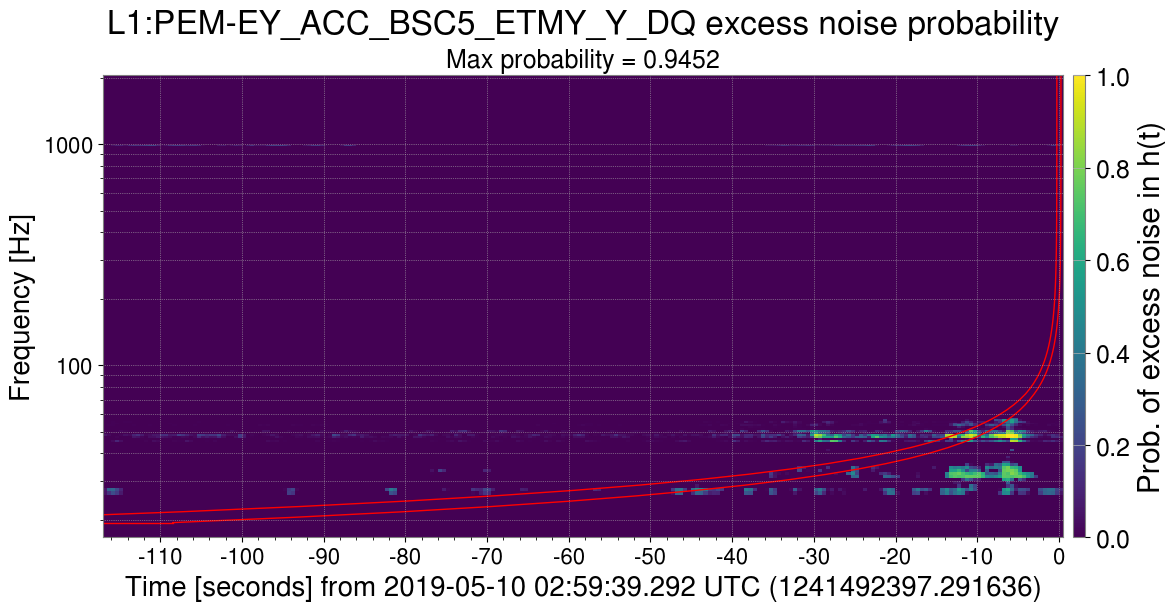
\includegraphics[width=\textwidth]{figures/noise-studies/vetting-spectrogram1.png}
	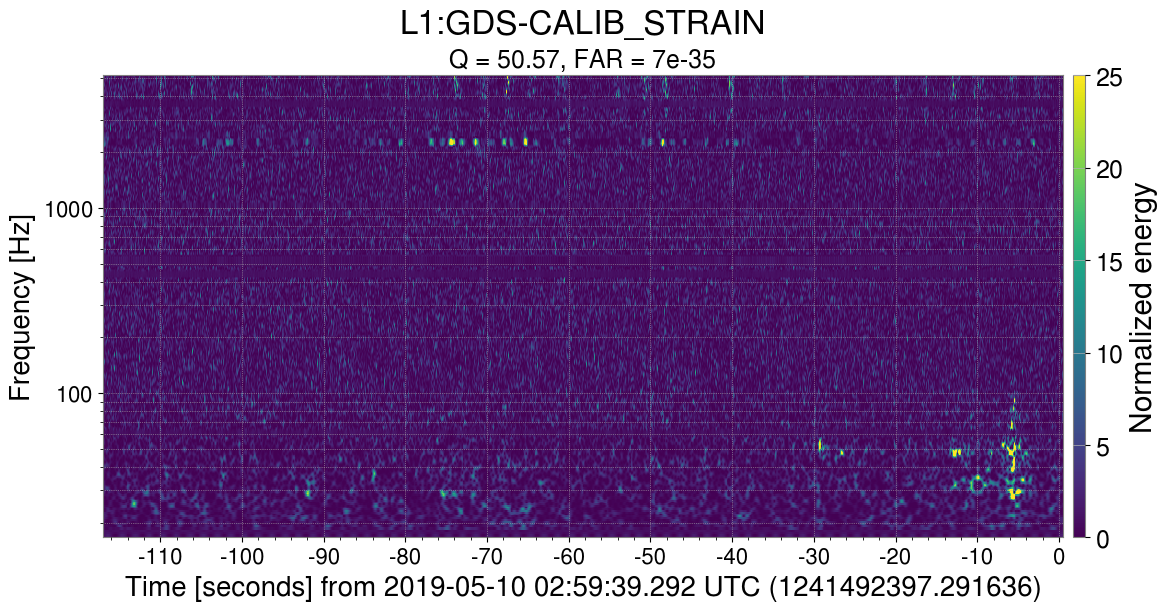
\includegraphics[width=\textwidth]{figures/noise-studies/vetting-spectrogram2.png}
	\caption
	[Probability spectrogram of an ETMY accelerometer at LLO and a constant-Q transform of the GW strain channel]
	{
		Probability spectrogram of an ETMY accelerometer at LLO (top) and a constant-Q transform of the GW strain channel (bottom).
		The red lines show the time-frequency path of GW event candidate S190510g.}
	\label{fig:vetting-spectrograms}
\end{figure}

Figure~\ref{fig:vetting-spectrograms} provides an example of a probability spectrogram output by \code{pemcheck} for an \ac{O3} \ac{GW} event candidate, S190510g.
The candidate signal coincides with scattering noise produced at the \ac{LLO} Y-end station by a thunderstorm.
The coupling projection predicts a peak probability of 0.87, meaning there is an 87\% probability that noise is present in the interferometer overlapping the time-frequency window of the \ac{GW} event.

There are still limitations to how well this method can predict the presence of excess noise in the \ac{GW} channel, discussed below.

\subsubsection{Coupling function tuning}

Coupling function projections often overestimate the \ac{GW} background level for a number of reasons.
The most common causes are all linked to the fact that coupling functions can only be measured during extended periods of detector maintenance, usually at the start of an observing run, leaving them vulnerable to becoming outdated as noise sources are introduced, changed, or mitigated.
If a noise source is introduced near a sensor, such as through the installation of new hardware, the sensor ambient can increase dramatically whether or not the noise source actually couples to the \ac{GW} channel.
If the new noise does not couple, then the projection overestimates the detector amplitude, leading to a spurious claim that a \ac{GW} candidate signal may be affected by environmental noise.
Conversely, if an existing noise source is removed or its coupling mechanism mitigated, then the \ac{GW} background drops, potentially below the level of estimated ambient noise projections.

For these reasons, coupling functions must be tuned to account for overestimated noise in the time around an event candidate.
This is done by simply treating background noise in a long stretch of time before the candidate as if it were a new injection.
Rather than re-measuring the coupling function, we can check for frequencies where projections estimate ambient coupling to exceed the \ac{GW} background, dividing the coupling function by the ratio by which it is overestimating.
The result is a coupling function that at most projects noise at background levels.

\begin{figure}
	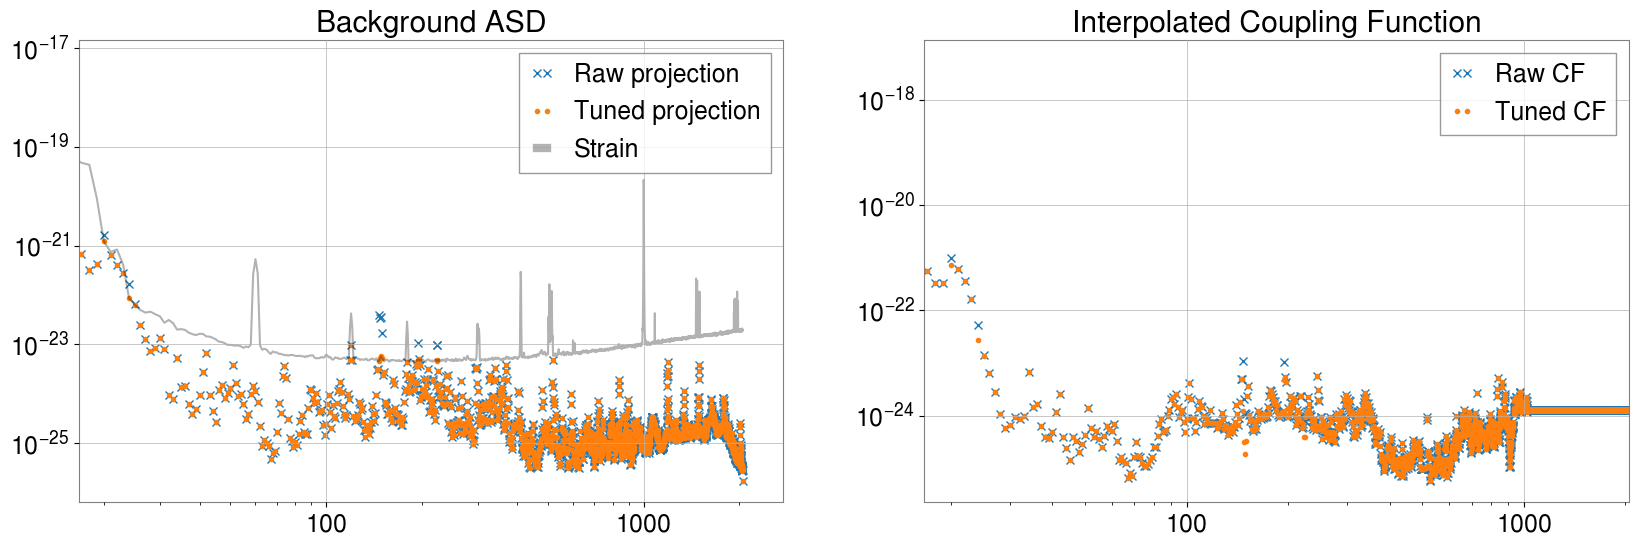
\includegraphics[width=\textwidth]{figures/noise-studies/vetting-tuning1.png}
	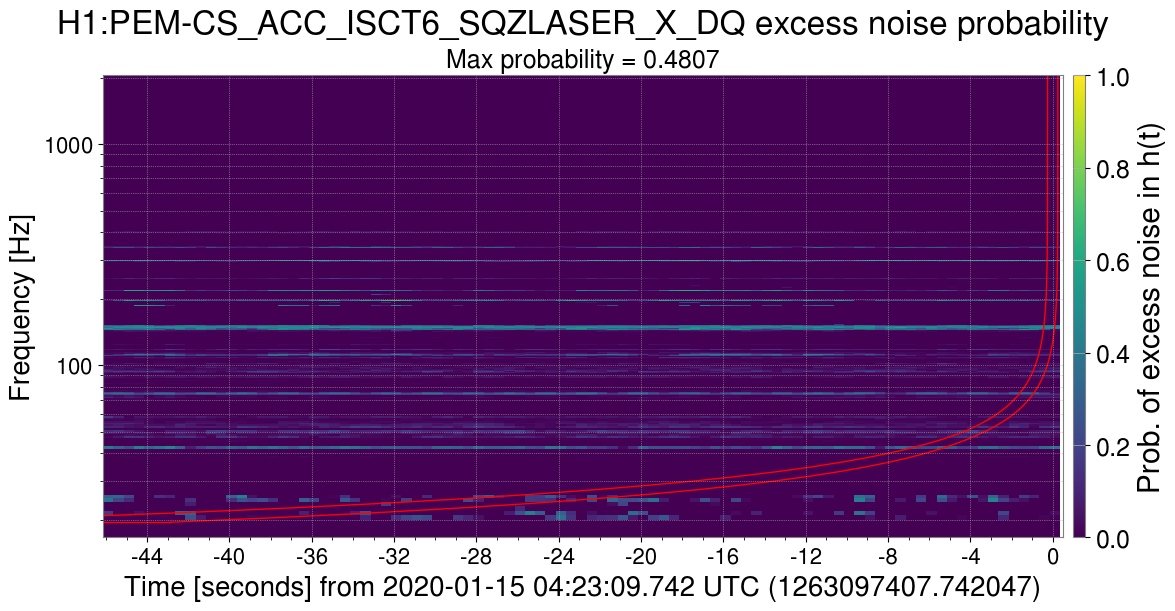
\includegraphics[width=\textwidth]{figures/noise-studies/vetting-tuning2.png}
	\caption
	[Coupling function tuning and the resulting probability spectrogram]
	{
		Coupling function tuning (top) and the resulting probability spectrogram (bottom).}
	\label{fig:vetting-tuning}
\end{figure}

Figure~\ref{fig:vetting-tuning} shows an egregious case of projected noise for an accelerometer on the squeezed light optics table overestimating the strain background amplitude.
The tuning reduces this to match the strain background, and the resulting probability spectrogram does not estimate a significant probability that excess noise is present.


\subsubsection{Grouping nearby sensors}

Even after tuning coupling functions, projections can still be overestimated in the presence of short duration ($\leq$ 1\,s) transients that are not likely to couple based on physical reasons.
Rack magnetometers (placed on the metal racks that hold the various control systems, data acquisitions systems, and power supplies in the electronics rooms) observe the highest rates of localized short-duration transients, routinely picking up magnetic fields from changes in nearby currents.
When these glitches coincide with a \ac{GW} event candidate they predict a probability of excess noise usually above 90\%.
Although the coincident rate is low for typical (\ac{BBH}) events, a long-duration \ac{GW} signal such as a \ac{BNS} will typically overlap with at least a few electronics glitches.

Since coupling functions are only intended to be used for noise sources distant from the sensors, projections from sensors placed close to each other ($\lesssim$ 1\,m) should be highly correlated if the input noise is environmental and not local to the individual sensors.
To incorporate this knowledge, \code{pemcheck} groups together magnetometers in each electronics room; their probability spectrograms are stacked and a pixel-wise minimum is computed to generate a combined group spectrogram.
This suppresses signals that project above the strain background in one magnetometer but not the others, so the projected excess noise probabilities are much lower than any of the peak probabilities reported by the individual sensors.
